\documentclass[journal]{IEEEtran}
\usepackage[T1]{fontenc}
\usepackage{amsmath,amssymb}
\usepackage{graphicx}
\usepackage{booktabs}
\usepackage{multirow}
\usepackage{makecell}
\usepackage[table]{xcolor}
\usepackage{pifont}
\usepackage{tikz}
\usetikzlibrary{positioning,arrows.meta,fit,calc}
\usepackage{cite}
\usepackage[hidelinks]{hyperref}
\usepackage[capitalise,nameinlink]{cleveref}

\newif\ifdraft
\draftfalse
\newcommand{\mini}{\ensuremath{{}^{\dagger}}}
\newcommand{\cmark}{\ding{51}}
\newcommand{\xmark}{\ding{55}}
\newcommand{\partialmark}{($\checkmark$)}
\ifdraft\newcommand{\todo}[1]{\textcolor{red}{[#1]}}\else\newcommand{\todo}[1]{}\fi
\input{numbers.tex}
\input{pending.tex}
\newcommand{\RQ}[1]{\textbf{RQ#1}}
\makeatletter\newcommand{\tabinput}[1]{\@@input #1 }\makeatother

\begin{document}

\title{Seen but Barely Used: Concept-Level Interpretability of Pedestrian Perception in a Sparse End-to-End Driving Model}

\author{Pavan~Yadav~Annappa%
\thanks{P.~Y.~Annappa is with the Pattern Recognition Lab, Friedrich-Alexander-Universit\"at Erlangen-N\"urnberg (FAU), 91058 Erlangen, Germany (e-mail: pavanyadava07@gmail.com).}}

\markboth{Preprint}{Annappa: Concept-Level Interpretability of Pedestrian Perception}

\maketitle

\begin{abstract}
Planning and closed-loop scores do not show whether an end-to-end driving model perceives pedestrians, what it
encodes about them, or whether its plan depends on them. We open the object queries of SparseDrive, a sparse
query-based end-to-end model, and trace pedestrians from image evidence to the planner on nuScenes, NAVSIM and
Bench2Drive/CARLA. The pedestrian class is a nearly orthogonal direction in query space; a sparse autoencoder spreads
it over about \NpedUnits{} units whose subspace, but not whose individual units, recurs across training seeds.
Walking towards the ego path or standing on a zebra crossing is linearly encoded beyond geometric confounds, yet such
pedestrians receive no more planner attention than others. Occlusion lowers the pedestrian logit at matched distance
and size, occluded pedestrians are recovered through the query memory, and newly appearing pedestrians are rarely
detected (first-sighting recall \FanOccZero{} occluded, \FanVisZero{} visible). Planner attention ranks the agents
whose removal moves the plan (rank-AUC \AucAttn), but removing a pedestrian from attention and collision rescoring
moves the plan by centimetres, and attention masking moves it less than for a matched car. Removing all detected
pedestrians from attention, rescoring and planner memory in every frame changes the plan about a sixth as much as
removing all vehicles; on NAVSIM this removal leaves the driving score unchanged for pedestrians (EPDMS \NavDPeds) but
lowers it for vehicles (\NavDVehicles). The pipeline uses only public code and data, and we discuss the implications for
safety argumentation.
\end{abstract}

\begin{IEEEkeywords}
Autonomous driving, explainable AI, interpretability, pedestrian detection, sparse autoencoders, concept activation vectors.
\end{IEEEkeywords}

% =====================================================================================================
\section{Introduction}
\IEEEPARstart{E}{nd-to-end} (E2E) driving models map camera images to a planned trajectory and are compared by
open-loop displacement error, by the NAVSIM score~\cite{dauner2024navsim} or by closed-loop driving
scores~\cite{jia2024bench2drive}. These numbers say how well a model drives on average. They do not say whether it
perceived a pedestrian, what it encoded about that pedestrian, or whether the plan would change if the pedestrian were
not there. For vulnerable road users this is the question a safety case under frameworks such as
SOTIF~\cite{iso21448} or UL~4600~\cite{ul4600} must answer, and it requires looking inside the
model~\cite{kuznietsov2024xaireview,atakishiyev2025safety}.

Recent work approaches E2E models from two sides. Planner-level concept discovery learns a sparse dictionary on the
latent space of a trajectory-scoring planner and edits it to change driving behaviour~\cite{motzkus2026drivingwrongway}.
Input-level audits remove objects from images or test for spurious cues and measure the plan
change~\cite{yang2026beyondleaderboard,cvaa2026,cadet2026}; on NAVSIM, planners rarely react to a removed
pedestrian~\cite{yang2026beyondleaderboard}. Neither side asks how the \emph{perception} part of the model represents a
pedestrian, which of its properties it encodes, and through which routes that representation reaches the plan.

Query-based E2E models make this tractable. In SparseDrive~\cite{sun2024sparsedrive} every road user is one object
query, a 256-dimensional feature refined over six decoder layers, carried to the next frame and read by the planner.
We use these queries as the unit of analysis and ask five research questions:
\begin{itemize}
\item[\RQ1] Where in the image does the evidence for a pedestrian come from, and which attribution maps can be trusted?
\item[\RQ2] How is ``pedestrian'' represented, and which finer pedestrian concepts are encoded beyond geometric confounds?
\item[\RQ3] What role does occlusion play, and how does the model detect pedestrians it cannot see?
\item[\RQ4] Does the planner use pedestrian queries, through which routes, and does its attention identify the ones that matter?
\item[\RQ5] Do the findings transfer to another dataset and camera rig (NAVSIM), and what does closed loop (CARLA) show?
\end{itemize}

\noindent Our contributions are:
\begin{enumerate}
\item An instance-level interpretability protocol for query-based E2E models: read-out points, query-to-annotation
matching, safety strata, causal interventions that close every planner-side route (attention, collision rescoring,
temporal memory) on cached perception, and scene-clustered statistics, implemented as a resumable pipeline built only
from public code and data (\cref{sec:method}).
\item A concept analysis of pedestrian perception combining class directions, control-task probes, TCAV, sparse
autoencoders with specificity controls, and fine-grained concepts tested against their confounds with LEACE
separability (\cref{sec:rq2,sec:rq3}).
\item A causal account of pedestrian reliance: attention points to the pedestrians that matter, but removing a pedestrian
from attention and rescoring moves the plan by centimetres, and attention masking moves it less than for a matched car; group removal that also closes
the memory route shows the same ordering, and a rare mode-switching tail carries the large effects (\cref{sec:rq4}).
\item Tests of the account on NAVSIM and in CARLA closed loop, including a Bench2Drive fine-tune with OpenDRIVE-derived
map labels, and a test of detection at first appearance (\cref{sec:rq3,sec:rq5}).
\end{enumerate}

\begin{figure*}[t]
\centering
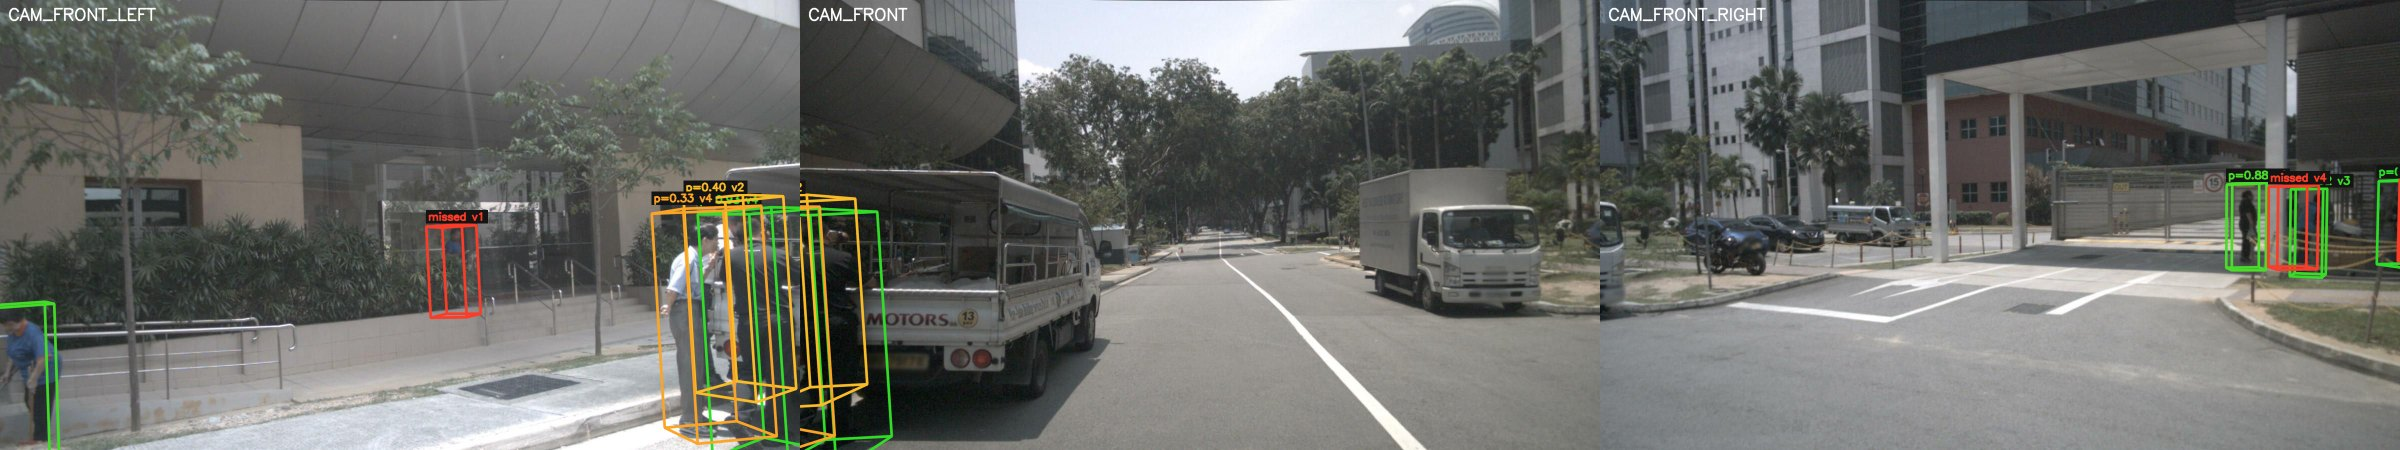
\includegraphics[width=\textwidth]{figures/f1_frame.jpg}
\caption{One nuScenes validation frame (front-left, front, front-right cameras) with every annotated pedestrian
coloured by the model's pedestrian probability $p$ for the matched query; red = no query with maximum class score
above 0.3 within 2\,m; v = visibility level (1: 0--40\,\%, 4: 80--100\,\%). Pedestrians next to the parked truck are
only weakly detected, one behind glass is missed, and on the right a fully visible pedestrian is missed between two
detected ones.}
\label{fig:teaser}
\end{figure*}

% =====================================================================================================
\section{Related Work}
\textbf{End-to-end driving and query-based perception.} Planning-oriented models such as UniAD~\cite{hu2023uniad},
VAD~\cite{jiang2023vad} and SparseDrive~\cite{sun2024sparsedrive} share one network for detection, tracking, mapping,
motion prediction and planning~\cite{chen2024e2esurvey}. SparseDrive builds on the sparse, temporally propagated
queries of the Sparse4D family~\cite{lin2022sparse4d,lin2023sparse4dv3} and of StreamPETR~\cite{wang2023streampetr},
which sample image features with deformable attention~\cite{zhu2021deformable}. Open-loop planning metrics on nuScenes
can be matched by models that use ego status alone~\cite{zhai2023admlp,li2024egostatus}, a shortcut that also bounds
how much any perceived agent can matter to the plan; imitation learning is prone to such causal
confusion~\cite{dehaan2019causalconfusion,codevilla2019limitations}, and end-to-end CARLA agents carry comparable hidden
biases~\cite{jaeger2023hiddenbiases}.

\textbf{Explaining driving models.} Early work visualised attention of image-to-steering
networks~\cite{kim2017causalattention}, and PlanT reads the attention of an object-level planner to identify the relevant
agents~\cite{renz2022plant}; recent models are trained for sparse, localised feature
maps~\cite{mirzaie2025interpretable}. Object-level counterfactual explanations edit
scene objects in image space~\cite{jacob2022steex,zemni2023octet}; counterfactual audits remove or re-light objects and
read the plan change~\cite{yang2026beyondleaderboard,cvaa2026} or audit reliance on spurious cues~\cite{cadet2026}. Closest to us,
Motzkus and Bernhard learn sparse dictionaries on the latent space of a trajectory-scoring planner and intervene on
concepts to improve the NAVSIM score~\cite{motzkus2026drivingwrongway}. We work one level earlier, on the perception
queries the planner reads, focus on pedestrians, control concepts for confounds, and close every planner-side route
when testing reliance.

\textbf{Concepts, units and interventions.} Linear probes~\cite{alain2016probes} with control
tasks~\cite{hewitt2019control} test decodability; TCAV~\cite{kim2018tcav} tests whether a direction moves a class
logit; LEACE~\cite{belrose2023leace} erases a concept linearly. Unit-level concept discovery goes back to Network
Dissection~\cite{bau2017netdissect} and ACE~\cite{ghorbani2019ace}; sparse autoencoders (SAEs) decompose superposed
features~\cite{elhage2022superposition} into sparse units~\cite{bricken2023monosemanticity,gao2025sae}, archetypal
variants stabilise them~\cite{fel2025archetypal}, and their units can depend on the random
seed~\cite{paulo2025saeseeds}. Our planner interventions are activation patching in the sense of causal mediation
analysis~\cite{vig2020mediation,meng2022rome}; patching and steering along a subspace can produce effects through
off-manifold directions~\cite{makelov2024illusion}, which is why we pair steering with norm-matched random directions. Whether attention explains a decision is
contested~\cite{jain2019attention,wiegreffe2019attention}; we test it causally for a planner. Probing has shown that 2D
detection transformers encode 3D object properties~\cite{probingdetr2026}.

\textbf{Evaluating attribution.} Gradient saliency~\cite{simonyan2014saliency}, SmoothGrad~\cite{smilkov2017smoothgrad}
and D-RISE~\cite{petsiuk2021drise} are evaluated with ROAD~\cite{rong2022road} and model-randomisation sanity
checks~\cite{adebayo2018sanity}.

\begin{table}[t]
\centering
\caption{Positioning against the closest recent work. \cmark{} yes, \partialmark{} partly, -- no. CVAA analyses
representations after input edits but not concepts, and selects objects but not pedestrians specifically.}
\label{tab:positioning}
\footnotesize
\resizebox{\columnwidth}{!}{%
\begin{tabular}{@{}lccccc@{}}
\toprule
 & \makecell{inside\\perception} & \makecell{pedestrian\\focus} & \makecell{concept\\discovery} & \makecell{confound\\control} & \makecell{closed\\loop} \\
\midrule
Motzkus \& Bernhard~\cite{motzkus2026drivingwrongway} & -- (planner) & -- & \cmark & -- & \partialmark \\
Yang et al.~\cite{yang2026beyondleaderboard} & -- (input edits) & \cmark & -- & -- & -- \\
CVAA~\cite{cvaa2026} & \partialmark & \partialmark & -- & -- & -- \\
\textbf{Ours} & \cmark & \cmark & \cmark & \cmark & \partialmark \\
\bottomrule
\end{tabular}}
\end{table}

% =====================================================================================================
\section{Model and Read-Out Points}\label{sec:model}
We analyse the released SparseDrive-S stage-2 checkpoint~\cite{sun2024sparsedrive} without modification. On nuScenes
validation~\cite{caesar2020nuscenes} it gives NDS \NDS, mAP \mAP, map mAP \mAPmap, AMOTA \AMOTA, planning L2
\PlanLtwo\,m and collision rate \PlanCol\,\%, within 0.01 of the values reported in the authors' repository.
\Cref{fig:arch} shows the parts we read and intervene on. A ResNet-50 with FPN encodes six cameras; the detection
decoder refines 900 object queries over six layers, each sampling image features around the query's 3D anchor with
deformable attention and attending to the other queries and to the instance bank; 600 queries are carried to the next
frame (the detector's memory). The planner prepends an ego query to the 50 highest-scoring agent queries; in each
planner layer the agents and the ego query attend to each other, to map queries and to a temporal queue holding their
own features of the previous three frames (for the ego query, its post-planner features). The planner outputs six
trajectory modes per driving command; a collision-aware rescoring penalises modes whose path overlaps the predicted
motion of any detection with score $\geq0.5$, and the best remaining mode is returned (3\,s, 6 waypoints).

\begin{figure}[t]
\centering
\begin{tikzpicture}[font=\scriptsize, node distance=3.0mm,
  blk/.style={draw, rounded corners=1.5pt, align=center, minimum height=6.5mm, inner sep=2pt, fill=gray!8},
  ro/.style={circle, draw=orange!80!black, fill=orange!20, inner sep=0.6pt, font=\tiny\bfseries},
  ar/.style={-{Stealth[length=1.6mm]}, thick}]
\node[blk] (cam) {6 cameras};
\node[blk, right=of cam] (bb) {ResNet-50\\+ FPN};
\node[blk, right=of bb] (det) {detection decoder\\900 queries $\times$ 6};
\node[blk, below=6mm of det] (bank) {instance bank\\(detector memory)};
\node[blk, right=7mm of det] (plan) {planner\\ego + top-50};
\node[blk, below=6mm of plan] (q) {temporal queue\\(planner memory)};
\node[blk, right=3mm of plan] (rs) {rescore\\+ select};
\draw[ar] (cam) -- (bb); \draw[ar] (bb) -- (det); \draw[ar] (det) -- (plan); \draw[ar] (plan) -- (rs);
\draw[ar] ([xshift=-4mm]det.south) -- ([xshift=-4mm]bank.north); \draw[ar] ([xshift=4mm]bank.north) -- ([xshift=4mm]det.south);
\draw[ar] ([xshift=-4mm]plan.south) -- ([xshift=-4mm]q.north); \draw[ar] ([xshift=4mm]q.north) -- ([xshift=4mm]plan.south);
\node[ro] at ($(det.north)+(-6mm,1.3mm)$) {1};
\node[ro] at ($(det.north)+(0mm,1.3mm)$) {2};
\node[ro] at ($(det.north)+(6mm,1.3mm)$) {3};
\node[ro] at ($(bank.west)+(-1.5mm,0)$) {4};
\node[ro] at ($(plan.north)+(0,1.3mm)$) {5};
\node[ro] at ($(q.west)+(-1.5mm,0)$) {6};
\node[ro] at ($(rs.north)+(0,1.3mm)$) {7};
\end{tikzpicture}
\caption{SparseDrive and our read-out points: \textbf{1} deformable sampling (attribution); \textbf{2} per-layer query
features (probes, TCAV, SAEs, concepts); \textbf{3} class head (class directions); \textbf{4} detector memory (history
ablation); \textbf{5} planner attention (masking, dropping, feature replacement, relocation); \textbf{6} planner memory;
\textbf{7} collision rescoring. Routes 5--7 are closed together in the complete-removal experiment.}
\label{fig:arch}
\end{figure}

% =====================================================================================================
\section{Method}\label{sec:method}
\subsection{Instances, matching and strata}
Each nuScenes pedestrian annotation within 50\,m with at least one lidar or radar point is matched to at most one
query by Hungarian assignment on the BEV centre distance (threshold 2\,m) among queries whose maximum class score
exceeds 0.3. Matching is class-agnostic, so a matched pedestrian may be classified as another class. The validation
split contains \NvalPed{} pedestrian annotations, of which \ValPedRecall{} are matched. Strata: \emph{visibility}
(nuScenes levels 1--2 = 0--60\,\%, 3--4 = 60--100\,\%), \emph{distance} ($<$15, 15--30, $>$30\,m) and \emph{corridor}:
ahead of the ego vehicle, within 8\,m of the expert future path and with a constant-velocity time-to-collision below
8\,s (\NcritWeight{} pedestrians). The corridor uses the expert's future path and is therefore an offline
stratification; a stricter variant (2.5\,m, 4\,s) contains \NcritStrict{} pedestrians.

\subsection{Notation}
For a plan $\hat{\tau}\in\mathbb{R}^{6\times2}$ and the unmodified plan $\tau$ of the same frame, the plan change is
$\Delta L_2 = \tfrac{1}{3}\sum_{t\in\{1,2,3\,\mathrm{s}\}}\lVert\hat{\tau}_t-\tau_t\rVert_2$; we also report the
longitudinal change at 3\,s, whether the selected mode switches, and the change of the minimum clearance to the
annotated future pedestrian boxes. For a concept direction $v$ and a pedestrian with layer-$l$ feature $h$ and final
pedestrian logit $z$, TCAV counts the fraction of pedestrians with $\nabla_h z\cdot v>0$. Rank-AUC treats the agents of
a stratum whose masking effect is in the top 20\,\% as positives and pools agents across frames. The steering strength
$\alpha$ scales a unit pedestrian direction to the mean norm of the top-10 pedestrian units' contribution
(\cref{sec:rq2}). Several ``pedestrian effects'' are reported and differ by population and intervention: all detected
pedestrian agents under attention masking (mean over every agent); GT-matched pedestrians in the matched comparison
with cars; corridor pedestrians under attention masking, rescoring removal or both; and whole-group removal per frame.

\subsection{Attribution (\RQ1)}
For a matched query we compute five maps of its pedestrian logit over the six images: the deformable-attention
sampling density (DFA), the input gradient~\cite{simonyan2014saliency}, SmoothGrad~\cite{smilkov2017smoothgrad}
($n{=}16$), gradient$\times$feature on the FPN features, and D-RISE~\cite{petsiuk2021drise} with 500 masks and a
mean-centred estimator (plain RISE sums are dominated by a constant and by mask-density noise). Faithfulness uses
ROAD~\cite{rong2022road}, with the noisy linear imputation approximated by Jacobi diffusion to the same harmonic
fixed point plus Gaussian noise (GPU-batched). Randomisation cascades from the last refinement layer towards the
backbone~\cite{adebayo2018sanity}; a method fails if its map at the last stage with finite activations keeps a Spearman
or SSIM similarity above 0.7. Label randomisation is replaced by a target-randomisation proxy (the map for another
class), run for the gradient and gradient$\times$feature.

\subsection{Concept analysis (\RQ2, \RQ3)}
\textbf{Class directions and probes.} We compare the final classifier's pedestrian weight with the other classes and
record which class wins for each matched pedestrian. Logistic-regression probes on layer-2, 4 and 6 query features are
trained on training scenes and tested on validation scenes (balanced accuracy). Selectivity is the plain accuracy
above a control task in which every tracked object keeps one random label~\cite{hewitt2019control}, computed on a
random frame split because objects must recur.

\textbf{TCAV.} For a concept we fit 30 concept activation vectors~\cite{kim2018tcav} on bootstrap samples of
training-split features and 30 random vectors on random partitions of the same pool, and take exact gradients of each
validation pedestrian's final logit with respect to its own layer-$l$ feature through all later decoder layers. Scores
are compared with Welch's t-test, Bonferroni-corrected over 12 tests (four concepts, three layers). For occlusion we
add two confound-controlled versions: occluded and visible sets matched cell by cell on distance and box height, and
features with distance and box height (linear and squared) regressed out.

\textbf{Sparse autoencoders.} We train TopK SAEs~\cite{gao2025sae} (2048 or 8192 units, $k\in\{16,32,64\}$) on
\SAEntrain{} layer-6 query features of the training split (score $>0.1$) and the dictionaries of the Overcomplete
toolbox~\cite{fel2025archetypal}. A dictionary is accepted if it explains $>$90\,\% of the variance with at most 64
active units and changes pedestrian AP by at most one point when its reconstruction is spliced into the live model
(centre-distance AP averaged over 0.5/1/2/4\,m on every fourth validation frame). Units are catalogued by the classes
of their 32 strongest activations; a unit is pedestrian-specific if at least 24 of them are pedestrians. For the
primary SAE (2048 units, $k{=}64$) we ablate the ten strongest pedestrian units, ten car units or ten random units, and
steer non-pedestrian queries along the pedestrian direction or a norm-matched random direction; stability is tested by
retraining with two further seeds.

\textbf{Fine-grained concepts.} From annotations, tracks and the nuScenes map we label ten contrasts among matched
pedestrian instance-frames of both splits (\cref{tab:concepts}). Each is tested with a probe on the features, a probe
on its confounds alone (the concept's distance, speed, visibility, box height or lateral offset, with squares), a probe
after regressing the confounds out of the features, and a shuffled-label control. A concept is encoded beyond its
confounds if the lower 95\,\% scene-bootstrap bound of the residual probe exceeds the shuffled control (or 0.5) by at
least five points; ``weak'' if it exceeds it by less. Separability uses LEACE~\cite{belrose2023leace}: erase concept A,
re-probe concept B, and report B's retained accuracy above chance (self-erasure is not reported, since the re-fitted
probe on erased features is ill-posed).

\subsection{Planner interventions (\RQ4)}
The deformable-aggregation kernel is non-deterministic (atomic additions), so re-running perception changes plans.
All planner interventions therefore re-run only the planner on cached perception, which makes the unmodified pass
bit-identical. Single-agent interventions on agent query $j$: masking $j$ as a key in the current frame's planner
attention; removing $j$ from the rescoring; both; dropping $j$ from the top-50; replacing its feature by the mean
pedestrian feature or another pedestrian's feature; and moving its anchor 3\,m into or out of the path (an
off-manifold probe, since the query feature still encodes the original position). \emph{Complete removal} closes all
planner-side routes for a group (all detected pedestrians, vehicles, or agents with score $>0.3$; queries below this
threshold are not removed, so the test covers confidently detected agents): the group is masked
from attention and removed from rescoring in every frame of the validation stream, and the masked pass is committed to
a separate planner memory, so that the ego history never attended to the group. Perception-side mixing (detector
self-attention, the image-derived ego feature) remains and is outside a planner-reliance claim. To test whether a
cheap signal predicts reliance we rank agents by ego-query attention, by the plan gradient (a first-order estimate of
the masking effect, used as an upper reference), by inverse time-to-collision (predicted agent velocity, constant ego
velocity) and randomly.

\subsection{Temporal ablation (\RQ3)}
The detector is re-run with its instance bank truncated to 0--3 frames of history (``full'' = the unbounded recurrent
bank), and with the detection head's temporal attention zeroed while keeping propagated queries. The first-appearance
test bins validation pedestrians by the number of earlier keyframes in which the same instance was annotated; the
first keyframe of each scene is excluded, since every pedestrian in it would count as newly appearing.

\subsection{External validity (\RQ5)}
\textbf{NAVSIM.} We run the nuScenes checkpoint zero-shot on NAVSIM navtest logs~\cite{dauner2024navsim} (camera mapping
to the nuScenes rig, 3\,s plans extended to 4\,s at constant velocity) and score with the official one-stage EPDMS.
Sensor data were available for 38 logs (selected by sensor availability on our mount, not by scenario content);
inference ran on \NavInferred{} of the \NavCached{} cached scenes, and after token filtering \NavN{} scenes from
\NavLogs{} logs are scored. Interventions: ``masked''/``dropped from top-50'' hide detected pedestrians in the last of the four history frames only (planner attention or top-50); the
complete-removal variants act in every frame, on memory and on rescoring, for pedestrians, vehicles or all agents. A
constant-velocity agent gives an ego-status reference.

\textbf{CARLA closed loop.} We fine-tune the checkpoint on 100 Bench2Drive clips~\cite{jia2024bench2drive}, without map
labels (map head frozen) and with map labels derived from the OpenDRIVE maps in SparseDrive's three classes (lane
dividers de-duplicated, road boundaries as the contour of the drivable-area union, pedestrian crossings including
those stored only as OpenDRIVE objects). All three models drive the 20 Bench2Drive routes with a pedestrian scenario
(pedestrian crossing, object crossing from behind an obstacle, parked-car crossing, pedestrian during a turn), twice
each, in CARLA 0.9.15~\cite{dosovitskiy2017carla}. Statistics use the route as the unit (paired, 10{,}000 bootstrap
resamples).

\subsection{Statistics and evaluated subsets}
CIs are 95\,\% cluster-bootstrap intervals over scenes (1{,}000 resamples) unless stated: the matched pedestrian--car
comparison uses 500 resamples, NAVSIM 2{,}000 over logs and CARLA 10{,}000 over routes. \Cref{tab:subsets} lists the
evaluated subset of every analysis; all use the full nuScenes v1.0-trainval split. Numbers are generated from the result files by a script, except the
attribution table and a few counts noted under Reproducibility.

\begin{table}[t]
\centering
\caption{Evaluated subsets (nuScenes v1.0-trainval; validation = 6{,}019 frames in 150 scenes).}
\label{tab:subsets}
\footnotesize
\begin{tabular}{@{}p{0.35\columnwidth}p{0.59\columnwidth}@{}}
\toprule
Analysis & Subset \\
\midrule
Matching, strata, class directions & all frames, both splits \\
Probes & 250{,}000 matched queries, both splits \\
SAE training / catalogue & 1.45\,M training queries / 0.5\,M \\
Attribution & 1 frame per validation scene (126 frames, 306 targets) \\
SAE splice, steering, controls & every 4th validation frame (1{,}505) \\
TCAV & every 3rd validation frame (\TcavN{} pedestrians) \\
Planner single-agent & every 3rd validation frame (2{,}007; 100{,}350 agents) \\
Complete removal & every validation frame (\SgNframes); table on frames with the group \\
Temporal ablation & every 6th validation frame \\
\bottomrule
\end{tabular}
\end{table}

% =====================================================================================================
\section{Results}
\subsection{\RQ1: Where the evidence comes from}\label{sec:rq1}
\Cref{tab:attr} and \cref{fig:attr} summarise \AttrN{} pedestrian targets. On corridor pedestrians, the DFA map, D-RISE
and gradient$\times$feature reach the lowest MoRF areas with overlapping CIs, so no single method is most faithful.
LeRF is saturated near 1 for all maps except D-RISE, which falls below random on it. The methods disagree: pixel rank
correlation is \RhoDfaGrad{} between DFA and the gradient and \RhoGradDrise{} between the gradient and D-RISE, while
the gradient family agrees internally (\RhoGradSmooth). DFA fails randomisation: its sampling locations follow the
anchor geometry, so it shows where the query looks rather than why it decides. SmoothGrad passes narrowly (last-stage
SSIM 0.695 against a 0.7 threshold, within noise of Gradient's 0.740 fail); D-RISE's pass is degenerate, because after randomising the last refinement layer
the reference detection no longer exists. Gradient maps are nearly identical for another target class, so they explain
``an object is here'' more than ``a pedestrian is here''. Qualitatively, the feature-based maps concentrate on the feet
and ground contact point, where a camera-only model can read depth.

\begin{table}[t]
\centering
\caption{Attribution on corridor pedestrians ($n{=}\AttrNcrit$; ROAD MoRF $\downarrow$, LeRF $\uparrow$, 95\,\% CI),
localisation on all \AttrN{} targets (pointing game, energy PG) and cascading randomisation (last valid stage:
$+$det-shared; D-RISE: blocks 1--6).}
\label{tab:attr}
\footnotesize
\setlength{\tabcolsep}{2.4pt}
\resizebox{\columnwidth}{!}{%
\begin{tabular}{@{}lccccc@{}}
\toprule
Method & MoRF & LeRF & PG & EPG & MPRT \\
\midrule
DFA & 0.47 [0.40, 0.53] & 0.98 & 0.82 & 0.54 & fail \\
Gradient & 0.64 [0.60, 0.69] & 1.00 & 0.56 & 0.10 & fail \\
SmoothGrad & 0.60 [0.55, 0.64] & 1.00 & 0.72 & 0.11 & pass$^a$ \\
Grad$\times$feat. & 0.50 [0.43, 0.55] & 0.99 & 0.66 & 0.15 & fail \\
D-RISE & 0.48 [0.44, 0.53] & 0.88 & 0.49 & 0.03 & degen.$^b$ \\
Random & 0.96 [0.95, 0.97] & 0.96 & 0.01 & 0.00 & -- \\
\bottomrule
\end{tabular}}\\[1pt]
{\scriptsize $^a$ last-stage SSIM 0.695 vs.\ threshold 0.7. $^b$ reference detection absent after randomisation.}
\end{table}

\begin{figure}[t]
\centering
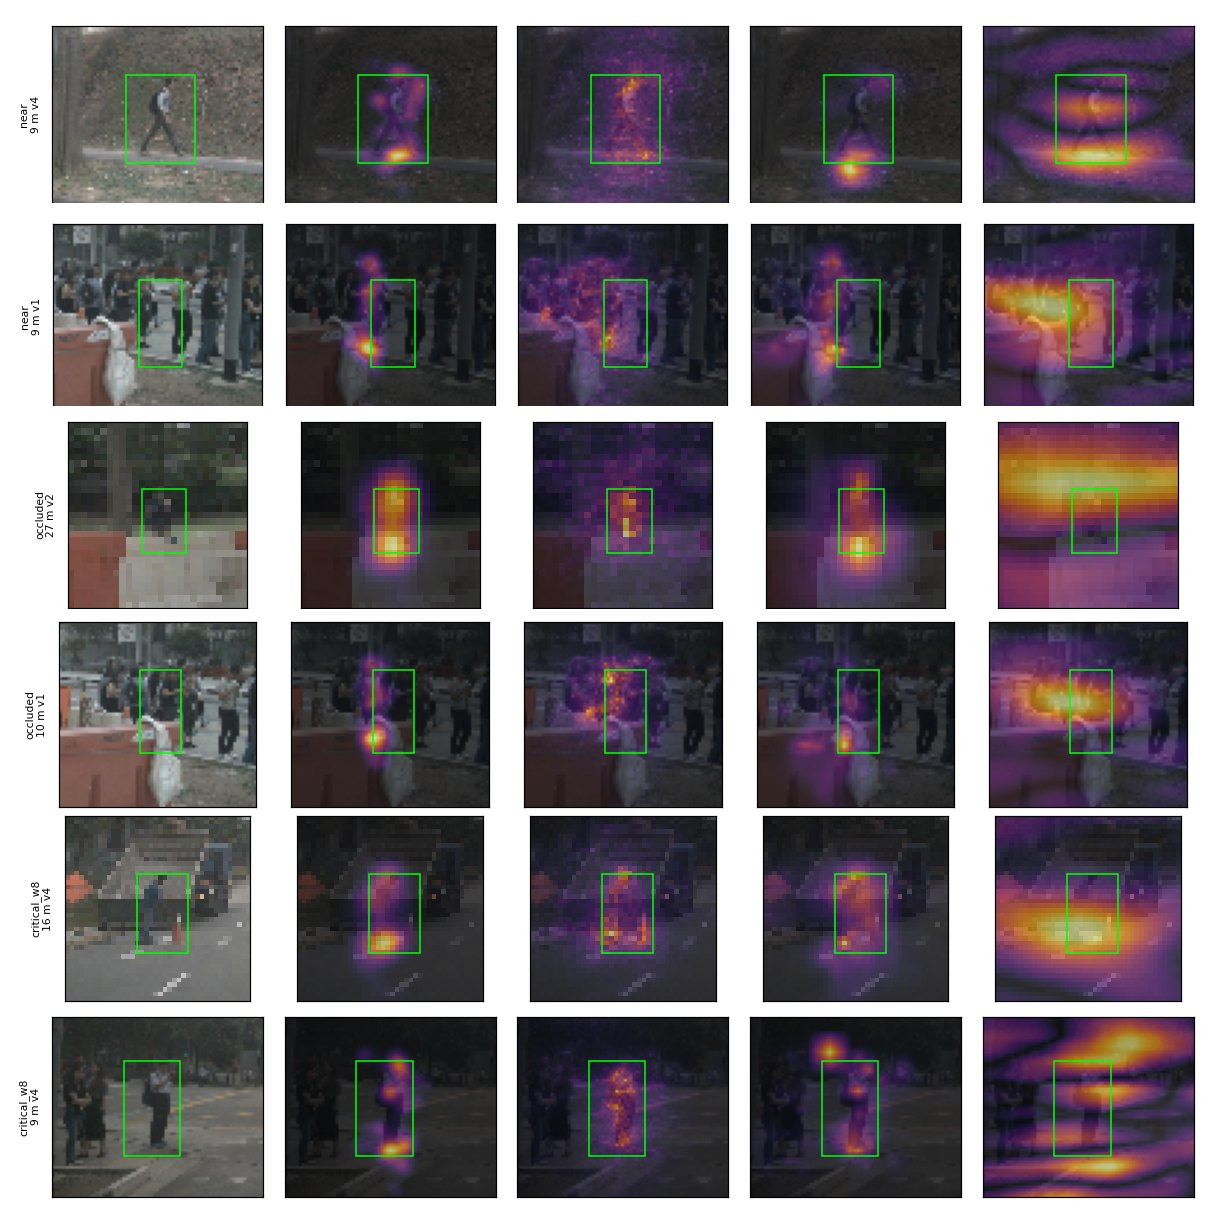
\includegraphics[width=\columnwidth]{figures/f2_attribution.jpg}
\caption{Attribution maps for six validation pedestrians (rows: two near, two occluded, two in the corridor).
Columns: input with annotated box, DFA, SmoothGrad, gradient$\times$feature, D-RISE (the plain gradient is close to
SmoothGrad and omitted). Banded D-RISE patterns are typical of a finite mask budget.}
\label{fig:attr}
\end{figure}

\subsection{\RQ2: How ``pedestrian'' is represented}\label{sec:rq2}
\textbf{A clean class direction.} The pedestrian weight vector is nearly orthogonal to every other class (largest cosine
\CosMax, with \CosMaxCls). Among the \ConfValN{} matched validation pedestrian instance-frames, \ConfVal\,\% are
out-scored by another class, most often by \RunnerUp{} (training split: \ConfTrain\,\%); since only \ValPedRecall{} of
validation pedestrians are matched, this statement covers the pedestrians the model localises. Probes read the class
from layer 2 on (\cref{tab:probes}). Distance and motion are decoded with similar balanced accuracy, whereas the
four-level visibility is weakly decodable. Corridor membership is highly imbalanced (majority share above 0.98 in the
strict corridor), so its plain-accuracy selectivity is capped and not informative.

\begin{table}[t]
\centering
\caption{Linear probes on query features, validation scenes (balanced accuracy, \%; chance = 100/k). Selectivity:
plain accuracy above the control task, frame split. Probe set: \ProbeN{} queries.}
\label{tab:probes}
\footnotesize
\setlength{\tabcolsep}{3pt}
\begin{tabular}{@{}lcccc@{}}
\toprule
Property ($k$ classes) & layer 2 & layer 6 & chance & selectivity \\
\midrule
\tabinput{tables/tab_probes.tex}
\bottomrule
\end{tabular}
\end{table}

\textbf{Pedestrian units.} The primary SAE explains \SAEev{} of the variance with 64 active units (\SAEdead\,\% dead).
\NdictPass{} dictionaries meet all three acceptance criteria (\cref{tab:sae}), including plain PCA, so reconstruction
quality alone does not establish concepts. \NpedUnits{} of \UnitsAlive{} live units are pedestrian-specific; in the
8192-unit SAE, 57 of 7{,}669 are (0.74\,\% vs.\ 1.00\,\%). Individual units are not stable across retraining:
with two further seeds the pedestrian units are matched with mean cosine \SeedPed{} (all units: \SeedAll), and only
\SeedPedMatched{} of \SeedPedN{} has a counterpart above 0.9 in both seeds (\SeedFigUnits{} of the three pedestrian units shown in
\cref{fig:units}), in line with~\cite{paulo2025saeseeds}. The concept is more stable than its units: every seed has a
similar number of pedestrian units (\SeedNped), their spans overlap with mean principal-angle cosine \SeedSub{}
(random unit sets of the same size: \SeedSubRand), and the pedestrian steering direction agrees with cosine \SeedDir.
The units in \cref{fig:units} are therefore examples from one seed, not identified features; in this seed they are
organised by viewing condition rather than pose: dim or distant pedestrians, close full-body walkers, pedestrians
standing in crowds.

Ablating the ten strongest pedestrian units costs \CtlPedPed{} pedestrian AP points and \CtlPedCar{} car points, and
moves the plan by \CtlPlanPed\,cm; ablating ten car units costs \CtlCarCar{} car and \CtlCarPed{} pedestrian points
(plan \CtlPlanCar\,cm), and ten random units cost \CtlRandPed{} and \CtlRandCar{} points (plan \CtlPlanRandAll\,cm for the
three random sets). The splice changes the perception of all agents, so its plan effect is not a test of planner
reliance on pedestrians.
Each set hurts its own class most, and random units do nothing, so the effect is class-selective rather than a generic
cost of removing ten units; the cross-class losses show that the strongest units also carry evidence shared between
object classes. Car units are chosen by car selectivity, computed exactly like pedestrian selectivity. Steering non-pedestrian queries along the pedestrian direction raises their
pedestrian logit by \StPedFourLogit{} at $\alpha{=}4$ (a norm-matched random direction: \StRandFourLogit), but the share
classified as pedestrian rises only from \StZero\,\% at $\alpha{=}0$ to \StPedFour\,\%: the units push the class
decision in the right direction without determining it.

\begin{table}[t]
\centering
\caption{Dictionaries on layer-6 query features: explained variance, active units, change of pedestrian AP when
spliced into the live model, acceptance.}
\label{tab:sae}
\footnotesize
\setlength{\tabcolsep}{4pt}
\begin{tabular}{@{}lcccc@{}}
\toprule
Dictionary & EV & L0 & $\Delta$AP$_\text{ped}$ & pass \\
\midrule
\tabinput{tables/tab_sae.tex}
\bottomrule
\end{tabular}
\end{table}

\begin{figure}[t]
\centering
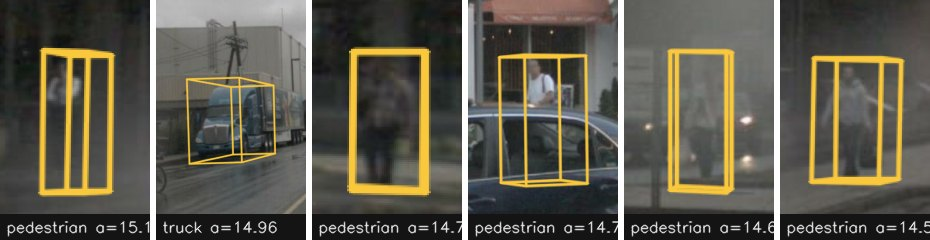
\includegraphics[width=\columnwidth]{figures/f4_latent_0.jpg}\\[1pt]
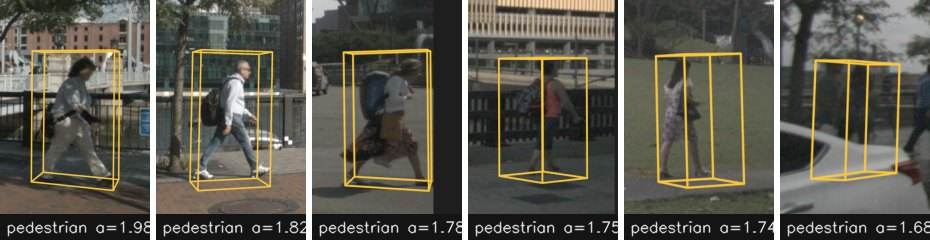
\includegraphics[width=\columnwidth]{figures/f4_latent_2.jpg}\\[1pt]
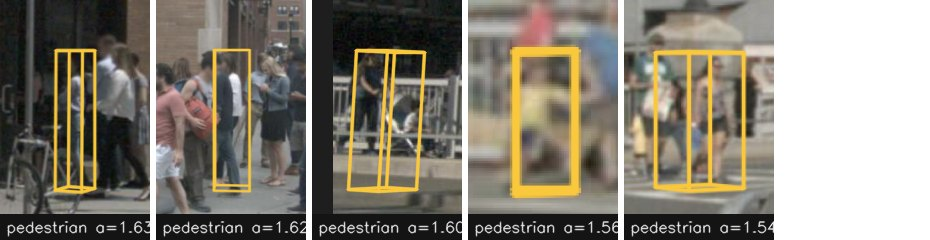
\includegraphics[width=\columnwidth]{figures/f4_latent_3.jpg}\\[1pt]
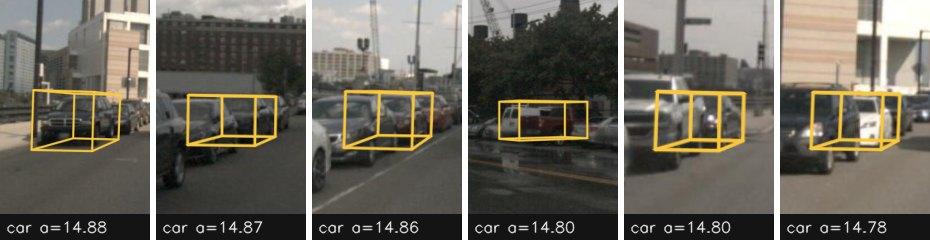
\includegraphics[width=\columnwidth]{figures/f4_latent_4.jpg}
\caption{Strongest activations of three pedestrian SAE units (rows 1--3: dim or distant pedestrians, with one truck
among the top activations; close full-body walkers; pedestrians standing in a crowd) and one car unit (row 4).
Training-set objects; $a$ = activation.}
\label{fig:units}
\end{figure}

\textbf{Fine-grained concepts.} \Cref{tab:concepts} separates what the queries encode about a pedestrian from what its
geometry implies. ``Moving'' is decodable but explained both by the annotated speed and by the model's own predicted
speed (residual \MovPredResid{} [\MovPredLo, \MovPredHi]): motion is represented through the velocity estimate.
\NStrictBeyond{} of the ten concepts are classed as beyond their confounds, among them walking towards the ego path, standing on a zebra
crossing, being on the road, being in a group, construction worker and emerging from occlusion; sitting is weak, and
child and night rest on few validation people (18 and 7) and are preliminary. The confound sets are geometric; for
walking towards the path the predicted velocity direction, and for road and zebra map-derived distances, would be
stricter controls that we have not run. Erasing any concept with LEACE keeps at
least 75\,\% of every other concept's above-chance accuracy, so they are separable. Being in a group pushes the
pedestrian logit up and moving and sitting push it down; walking towards the path is encoded but does not move the
class logit.

\begin{table*}[t]
\centering
\caption{Fine-grained pedestrian concepts. $n_\text{pos}$: matched instance-frames of both splits. Balanced accuracy
on validation scenes of probes on the features (feat), the confounds alone (conf) and the features with confounds
regressed out (resid). TCAV on the pedestrian logit, $^*$ significant after Bonferroni correction; the random-direction
means lie between 0.46 and 0.57. Verdict: strict criterion (\cref{sec:method}).}
\label{tab:concepts}
\footnotesize
\begin{tabular}{@{}lcccccl@{}}
\toprule
Concept (positive vs. negative) & $n_\text{pos}$ & feat & conf & resid & TCAV & verdict \\
\midrule
\tabinput{tables/tab_concepts.tex}
\bottomrule
\end{tabular}
\end{table*}

\subsection{\RQ3: Occlusion and memory}\label{sec:rq3}
\textbf{Occlusion is negative evidence.} In the last decoder layer the occluded-vs.-visible direction lowers the
pedestrian logit: TCAV \TcavOcc{} vs.\ \TcavOccRand{} for random directions (Bonferroni $p=\TcavOccP$,
\cref{tab:tcav}). The effect survives confound control: \OccMatched{} vs.\ \OccMatchedR{} with sets matched on distance
and box height, and \OccResid{} vs.\ \OccResidR{} with both regressed out. The direction reverses across layers (0.60
at layer 2), as does the corridor direction, which pushes towards the class in the last layer (0.74 vs.\ 0.50), a bias
in the safe direction. Together with the weak visibility probe this suggests that occlusion acts as evidence against
the class rather than being stored as an explicit value (\cref{fig:occ}).

\begin{table}[t]
\centering
\caption{TCAV on the pedestrian logit ($n$ = \TcavN{} validation pedestrians); Bonferroni over all 12 tests; the strict
corridor has few positives.}
\label{tab:tcav}
\footnotesize
\setlength{\tabcolsep}{2.6pt}
\begin{tabular}{@{}lccccc@{}}
\toprule
Concept & layer & TCAV & random & $p_\text{Bonf.}$ & sig. \\
\midrule
\tabinput{tables/tab_tcav.tex}
\bottomrule
\end{tabular}
\end{table}

\begin{figure}[t]
\centering
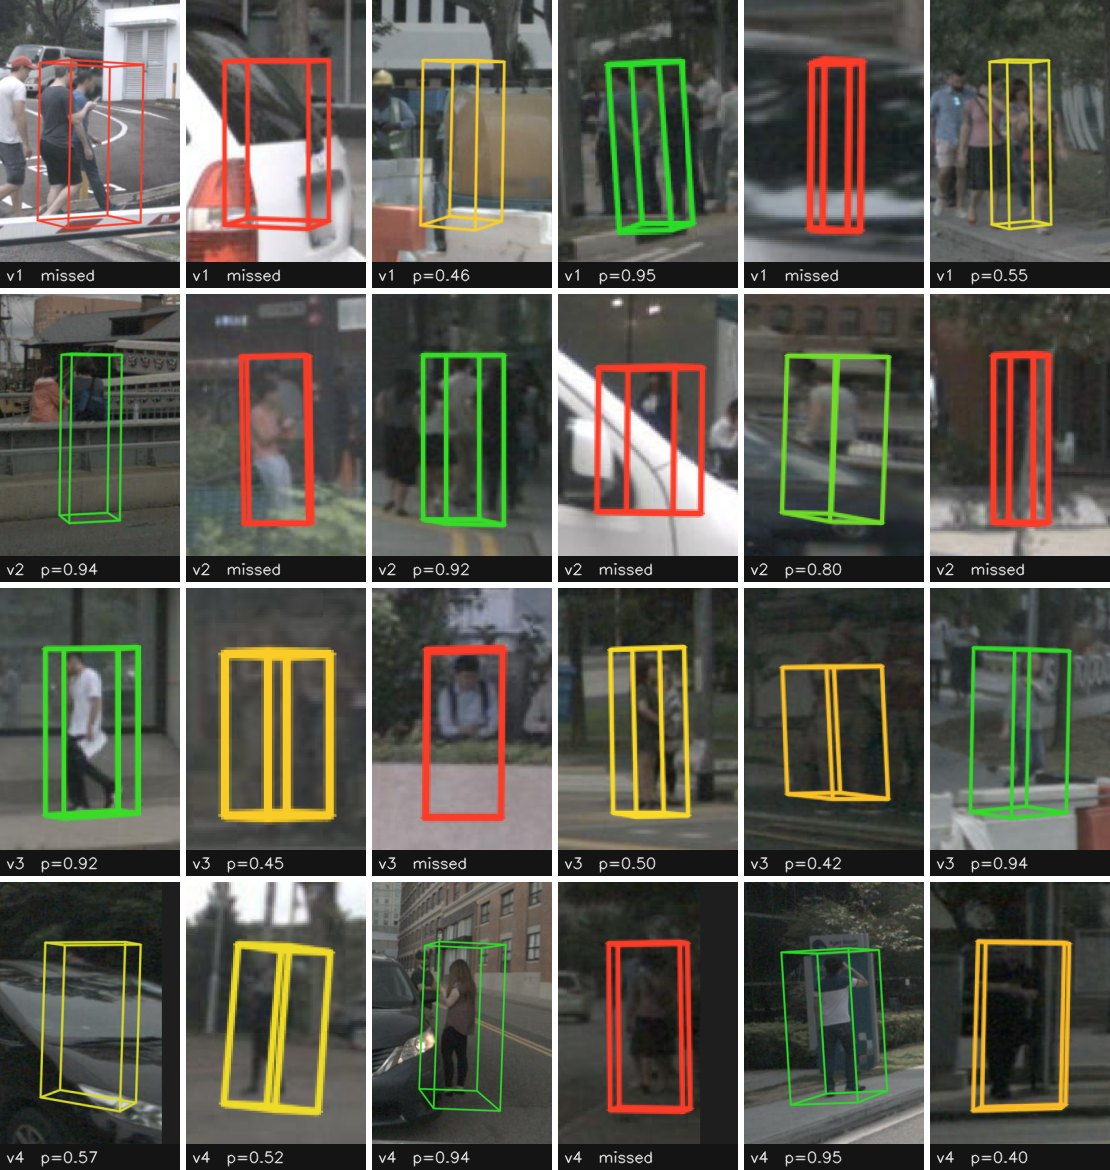
\includegraphics[width=\columnwidth]{figures/f3_occlusion.jpg}
\caption{Validation pedestrians closer than 30\,m, one row per visibility level (top: 0--40\,\%, bottom: 80--100\,\%),
coloured by pedestrian probability; ``missed'' = no query above 0.3 within 2\,m.}
\label{fig:occ}
\end{figure}

\textbf{Hidden pedestrians are found through memory.} Without history, recall falls from \MemFullOcc{}
[\MemFullOccLo, \MemFullOccHi] to \MemHnoneOcc{} for partly or heavily occluded pedestrians (visibility 0--60\,\%, $n$ =
\RecNocc) and from \MemFullVis{} to \MemHnoneVis{} for visible ones: a relative loss of \MemRelOcc\,\% vs.\
\MemRelVis\,\%, with a difference in absolute loss of \MemDid{} [\MemDidLo, \MemDidHi]. Recall rises monotonically with
0--3 frames of history (\cref{fig:memory}). Zeroing the detection head's temporal attention barely changes recall
(\RecDetTemp), so the memory is carried by the propagated queries. Newly appearing pedestrians are rarely
detected: excluding the first keyframe of each scene, where a pedestrian is ``first seen'' only because the scene starts,
recall at first sighting is \FanOccZero{} for heavily occluded and \FanVisZero{} for visible pedestrians, and it rises
to \FanOccFour{} and \FanVisFour{} after four or more earlier sightings. The penalty of a first sighting is not
specific to occlusion: the occlusion $\times$ first-sighting interaction is \FanInt{} [\FanIntLo, \FanIntHi]
(scene bootstrap; \FaInt{} [\FaIntLo, \FaIntHi] including scene starts).

\begin{figure}[t]
\centering
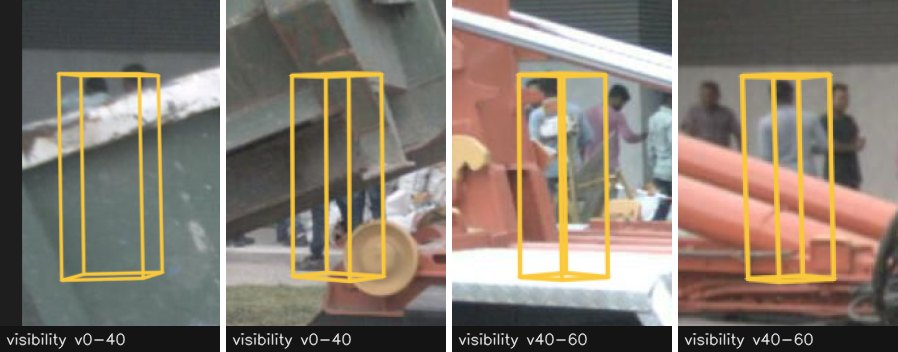
\includegraphics[width=0.8\columnwidth]{figures/f5_memory.jpg}\\[2pt]
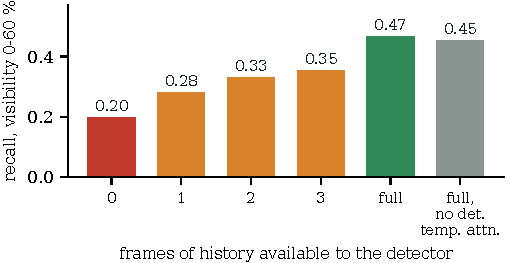
\includegraphics[width=\columnwidth]{figures/memory_recall.pdf}
\caption{Top: a pedestrian behind construction machinery over four keyframes (0.5\,s apart); in the last frame it is
detected only with $\geq$3 frames of history. Bottom: recall of heavily occluded pedestrians vs.\ history length.}
\label{fig:memory}
\end{figure}

\subsection{\RQ4: Does the planner use pedestrians?}\label{sec:rq4}
\textbf{Attention ranks the agents whose masking moves the plan.} For corridor pedestrians (8\,m / 8\,s stratum),
ego-query attention ranks the agents whose masking matters most with rank-AUC \AucAttn{} [\AucAttnLo, \AucAttnHi];
in the pre-specified strict stratum (2.5\,m / 4\,s) only \AucStrictN{} agents qualify and the AUC is uninformative
(\AucStrict{} [\AucStrictLo, \AucStrictHi]). Target and ranker share the attention pathway, so this AUC measures
consistency between attention and its own removal rather than independent relevance; the plan gradient, a first-order estimate of
the target, reaches \AucGrad. Inverse time-to-collision ranks them worse than chance in this stratum (AUC \AucPhys{}
[\AucPhysLo, \AucPhysHi]): more urgent corridor pedestrians move the plan less (Spearman \PhysRho{} between
1/TTC and the masking effect), so geometric urgency does not explain which pedestrians the planner uses. Randomising the planner lowers attention's AUC from \RandAllT{} to \RandAllR{} over all
agents and from \RandPedT{} to \RandPedR{} over pedestrians.

\textbf{Single pedestrians: attention and rescoring.} For the corridor pedestrians, masking from current attention moves the
plan by \SiAttn{} cm [\SiAttnLo, \SiAttnHi], removing from rescoring by \SiRs{} cm, and both by \SiBoth{} cm
[\SiBothLo, \SiBothHi] ($n$ = \SiN). The rescoring route is rarely active: in the existing rescore ablation \RsPen{} of
\RsN{} pedestrian agents change any penalty and \RsSel{} change the selected mode. Over all pedestrians the effect is
\MaskPedCm\,cm and flips the collision outcome in \MaskPedFlips{} of \MaskPedN{} cases. Relocating a pedestrian 3\,m
into the path (\RelocInto\,cm) and swapping its feature (\RelocSwap\,cm) move the plan by similar small amounts.

For scale, the planner's own average L2 error to the expert trajectory is \PlanLtwo\,m, so the mean single-pedestrian effect
(\ClsPedMean\,cm) is about 1\,\% of that error. We do not test the normative question of whether the planner should react more, e.g.
on frames where the expert yields to a pedestrian.

\textbf{Encoded concepts are not used preferentially.} \Cref{tab:conceptplanner} links each validation pedestrian to
its planner row by position and compares, within distance bins, the attention percentile and the masking effect of
pedestrians with and without a concept. Walking towards the ego path, being on a zebra crossing and being on the road,
all encoded beyond their confounds (\cref{tab:concepts}), receive neither more attention nor a larger masking effect;
emerging from occlusion and construction workers receive less attention, and pedestrians in groups move the plan less.

\begin{table}[t]
\centering
\caption{Concept $\rightarrow$ planner on validation pedestrians: positive minus negative attention percentile and
masking effect (cm), averaged over distance bins (0--15, 15--30, 30--100\,m); scene-bootstrap 95\,\% CIs.
$n_+$ = positive pedestrian-frames.}
\label{tab:conceptplanner}
\footnotesize
\setlength{\tabcolsep}{2pt}
\resizebox{\columnwidth}{!}{%
\begin{tabular}{@{}lccc@{}}
\toprule
Concept & $n_+$ & $\Delta$ attention pct. & $\Delta$ effect (cm) \\
\midrule
\tabinput{tables/tab_concept_planner.tex}
\bottomrule
\end{tabular}}
\end{table}

\textbf{Pedestrians vs.\ vehicles.} By predicted class, the mean single-agent effect is \ClsPedMean\,cm for pedestrians
against \ClsCarMean\,cm for cars and \ClsBusMean\,cm for buses, and the pedestrian median (\ClsPedMed\,cm) is the lowest
of all classes. Matching GT pedestrians and GT cars on distance, lateral offset to the path, detection confidence and
corridor membership (\MatchNstrata{} strata, \MatchNped{} pedestrians, \MatchNcar{} cars), a pedestrian moves the plan
by \MatchPed\,cm and a car by \MatchCar\,cm, a difference of \MatchDiff{} cm [\MatchDiffLo, \MatchDiffHi]. Group removal
shows the same ordering (\cref{tab:sustained}): on the \SgPedsNfr{} frames with at least one detected pedestrian,
removing all of them from attention, rescoring and memory in every frame moves the plan by \SgPedsFull{} cm
[\SgPedsFullLo, \SgPedsFullHi], against \SgVehFull{} cm for vehicles and \SgAgentsFull{} cm for all agents, with on
average \SgPedsPerFrame{} pedestrians and \SgVehPerFrame{} vehicles per frame. Per removed agent this is about 1\,cm for
pedestrians and 3\,cm for vehicles (a coarse normalisation, since group effects need not add up over agents). Closing the memory route adds little:
complete removal changes the plan only slightly more than masking pedestrians in the current frame (\SgPedsCur{} cm),
and in frames without a current pedestrian, where only the ego history differs, the change is \SgPedsAbsent{} cm. In
frames with a corridor pedestrian the effect of complete removal rises to \SgPedsFullCorr{} cm (mode switch in
\SgPedsFullCorrMode\,\%), and it changes the GT-collision outcome in \SgPedsColFlip\,\% of frames, against
\SgVehColFlip\,\% for vehicles.

\begin{table}[t]
\centering
\caption{Group removal over the validation split: plan change $\Delta L_2$ (cm, scene-bootstrap 95\,\% CI) on the
frames where the group is detected, when the group is masked from current-frame attention (cur), additionally removed from rescoring (+rs), or removed from attention,
rescoring and planner memory in every frame (complete).}
\label{tab:sustained}
\footnotesize
\setlength{\tabcolsep}{2pt}
\resizebox{\columnwidth}{!}{%
\begin{tabular}{@{}lcccc@{}}
\toprule
Group & frames & cur & +rs & complete \\
\midrule
\tabinput{tables/tab_sustained.tex}
\bottomrule
\end{tabular}}
\end{table}

\textbf{The tail.} Effects are skewed: the median single-pedestrian effect is \TailMed\,cm and the 99th percentile
\TailPnn\,cm, but \TailNfifty{} maskings move the plan by more than 0.5\,m, up to \TailMax\,m. All effects above
\TailNoSwitchMax\,cm involve a switch of the selected mode, which happens in \TailNmode{} of \MaskPedN{} maskings
(\TailModeRate\,\%; mean effect \TailModeMean\,m). Of these, \ModeSwMatched{} are GT-matched pedestrians at a median
\ModeSwDist\,m, \ModeSwCorr{} in the corridor, with median attention rank \ModeSwRank{} of 50. \Cref{fig:planner}
shows the frame whose top-attended pedestrian is fully visible; it is the largest effect without a mode switch, not the
largest effect overall.

\begin{figure}[t]
\centering
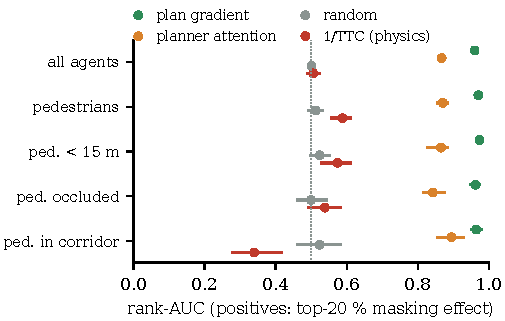
\includegraphics[width=\columnwidth]{figures/auc.pdf}
\caption{Rank-AUC of four rankers for identifying the agents whose masking moves the plan most (scene-bootstrap 95\,\% CIs).}
\label{fig:auc}
\end{figure}

\begin{figure}[t]
\centering
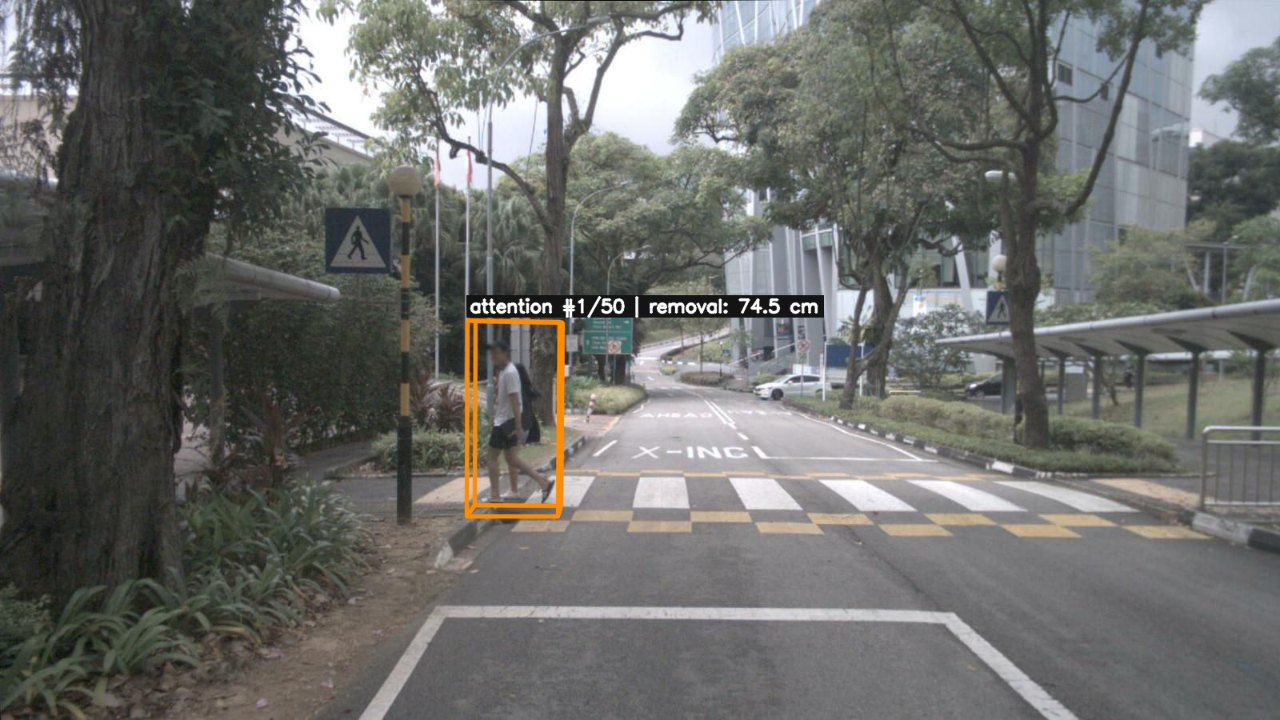
\includegraphics[width=\columnwidth]{figures/f6_planner.jpg}
\caption{A frame where the planner's top-attended agent of 50 is a fully visible pedestrian on a zebra crossing;
masking it moves the plan by 74.5\,cm without a mode switch, the largest such effect. Boxes are coloured by attention
rank; ``removal'' = plan change when the pedestrian is masked.}
\label{fig:planner}
\end{figure}

\subsection{\RQ5: External validity}\label{sec:rq5}
\textbf{NAVSIM.} Zero-shot, SparseDrive-S reaches EPDMS \NavEPDMS{} on \NavN{} scenes from \NavLogs{} navtest logs;
\NavAnyFault\,\% of the scenes with a detected pedestrian contain an at-fault collision. Masking all detected
pedestrians in the last frame changes the score on pedestrian scenes by at most \NavMaxDelta, and the changed collision
outcomes (11 fixed, 4 new when masked; 13 and 11 when dropped from the top-50) are not significant (sign test $p$ = \NavSignMaskP{} and
\NavSignDropP). \Cref{tab:navsim} adds complete removal (attention, rescoring and memory, in every history frame): EPDMS
\NavFullpeds{} with pedestrians removed, \NavFullvehicles{} with vehicles removed and \NavFullagents{} with all agents
removed, against \NavNone{} unchanged and \NavCv{} for a constant-velocity agent. With paired per-scene differences
and a log-clustered bootstrap (33 logs), removing vehicles lowers EPDMS by \NavDVehicles{}
[\NavDVehiclesLo, \NavDVehiclesHi] and the no-collision score by \NavDVehiclesNc{} (\NavDVehiclesNew{} new and
\NavDVehiclesFix{} avoided collisions), whereas removing pedestrians changes EPDMS by \NavDPeds{}
[\NavDPedsLo, \NavDPedsHi] and the no-collision score by \NavDPedsNc{} [\NavDPedsNcLo, \NavDPedsNcHi]
(\NavDPedsNew{} new, \NavDPedsFix{} avoided). On a second dataset and camera rig, the planner's score therefore
depends on vehicles; for pedestrians there is no evidence of degradation, and the no-collision shift towards fewer
at-fault collisions is borderline (sign test $p$ = 0.064; six group $\times$ metric comparisons, uncorrected). Without
pedestrian detection recall on OpenScene, which we do not report, this null cannot separate weak reliance from missed
detections.

\begin{table}[t]
\centering
\caption{NAVSIM one-stage EPDMS (zero-shot, \NavN{} scenes). Removal = group removed from planner attention,
rescoring and memory in every history frame. Pedestrian scenes: $\geq$1 detected pedestrian (\NavNped).
NC = no at-fault collision, EP = ego progress.}
\label{tab:navsim}
\footnotesize
\setlength{\tabcolsep}{5pt}
\begin{tabular}{@{}lcccc@{}}
\toprule
 & all & \multicolumn{3}{c}{pedestrian scenes} \\
\cmidrule(l){3-5}
Planner input & EPDMS & EPDMS & NC & EP \\
\midrule
\tabinput{tables/tab_navsim_groups.tex}
\bottomrule
\end{tabular}
\end{table}

\textbf{CARLA closed loop.} \Cref{tab:carla} reports the 20 pedestrian routes. With the route as the unit, both
fine-tunes complete less of the route than the zero-shot model (map labels: \CrMapZsRc{} points [\CrMapZsRcLo,
\CrMapZsRcHi]; no map labels: \CrEthZsRc{} [\CrEthZsRcLo, \CrEthZsRcHi]) and have fewer pedestrian collisions per run
(\CrMapZsPc{} [\CrMapZsPcLo, \CrMapZsPcHi] and \CrEthZsPc{} [\CrEthZsPcLo, \CrEthZsPcHi]); driving-score differences are
not resolved (map vs.\ zero-shot \CrMapZsDs{} [\CrMapZsDsLo, \CrMapZsDsHi]). A route stopped early meets fewer
pedestrians, so the collision reduction is largely a consequence of driving less. The zero-shot model, which completes
most routes, records \CrZsEvents{} pedestrian collisions in \CrZsRuns{} of its 40 runs; without a
closed-loop removal run this does not show whether it reflects weak reliance or missed detections. Pedestrian interventions in closed loop are left for future work.

\begin{table}[t]
\centering
\caption{CARLA closed loop on the 20 Bench2Drive pedestrian routes, two repetitions each (40 runs per model). DS =
driving score, RC = route completion (\%), succ.\ = success rate (\%); collisions are event counts over 40 runs.}
\label{tab:carla}
\footnotesize
\setlength{\tabcolsep}{2pt}
\resizebox{\columnwidth}{!}{%
\begin{tabular}{@{}lccccccc@{}}
\toprule
Model & runs & DS & RC & succ. & ped. & veh. & layout \\
\midrule
\tabinput{tables/tab_carla.tex}
\bottomrule
\end{tabular}}
\end{table}

% =====================================================================================================
\section{Discussion}
\textbf{Attention ranks, but does not measure, reliance.} The planner's attention predicts which agents matter
relative to each other, but not how much they matter: removing an attended pedestrian from attention and rescoring moves
the plan by centimetres, and closing the memory route as well does not change this. Attention maps of a planner therefore cannot serve as evidence that a pedestrian was taken into
account~\cite{jain2019attention,wiegreffe2019attention}; a causal test that closes all planner-side routes can, and it
is cheap on cached perception.

\textbf{Pedestrians are used less than cars.} At matched distance, path offset and confidence, and as a group, hiding
pedestrians changes the plan less than hiding cars or vehicles. This is consistent with an imitation-trained planner on
nuScenes, where the expert rarely yields to pedestrians, and with the ego-status shortcut~\cite{zhai2023admlp,li2024egostatus}.
The large effects are mode switches, a discrete and rare mechanism that a safety argument has to characterise rather
than average away.

\textbf{The weak point is first appearance.} The detector depends on its query memory, and a pedestrian that has
just appeared has no memory yet: excluding scene starts, only \FanOccZero{} of occluded and \FanVisZero{} of visible
pedestrians are detected at first sighting. Scenario-based testing (e.g. Bench2Drive's object-crossing
routes, where the zero-shot model collides in most runs) should concentrate here.

\textbf{Concept tests need confound control and data.} ``Moving'' is decodable but explained by speed; without the
confound-only and residual probes it would be reported as a learned concept. In a pilot on the two validation scenes of
nuScenes-mini (not reported here), several concepts appeared confound-explained that the full data show to be encoded, so
sample size is part of the protocol.

% =====================================================================================================
\section{Limitations}
We analyse one model, SparseDrive-S; the protocol applies to other query-based planners and extending it is the most
important next step. All nuScenes analyses are open loop, and the planner-reliance claims exclude perception-side
mixing. Labels come from annotations, tracks and HD maps; concept tests are linear. The NAVSIM evaluation is zero-shot
with a camera remapping on the \NavLogs{} navtest logs with complete sensor data. The CARLA fine-tunes use 100 clips,
closed-loop results vary between repetitions, and no pedestrian intervention was run in closed loop. Complete removal
covers detections with score above 0.3; sub-threshold pedestrian evidence stays in the planner, and we do not report
pedestrian detection recall on OpenScene. TCAV significance is computed over CAV refits against random CAVs, not over
pedestrians or scenes, so it states that a direction is consistent, not how much the effect varies across the population.

\section{Conclusion}
Opening the object queries of an end-to-end driving model shows a pedestrian representation that is clean, spread over a
subspace that is partly reproduced across seeds rather than by fixed units, sensitive to planning-relevant properties and supported by memory under occlusion, and a planner
that attends to the right pedestrians but relies on them less than on cars. Interventions that close every planner-side
route turn these observations into causal statements, which a safety argument for vulnerable road users needs.

\section*{Reproducibility}
The pipeline uses only the public SparseDrive code and checkpoint, nuScenes, NAVSIM/OpenScene, Bench2Drive and CARLA, and
is resumable across interruptions (PyTorch 1.13.1, mmcv 1.7.1, flash-attention planner; eager and flash planner outputs
agree to $10^{-3}$\,m). Numbers and tables are generated from the result files by \texttt{build\_numbers.py}; the attribution table
(\cref{tab:attr}) and a few in-text counts were transcribed from the generated report.
Camera images are from nuScenes (Motional), used under CC BY-NC-SA 4.0. Code: \url{https://github.com/pavanyadava007/seen-but-barely-used}.

\bibliographystyle{IEEEtran}
\bibliography{references}

\end{document}
